
\renewcommand{\thefigure}{\thesection \arabic{figure}}
\setcounter{figure}{0}



%%%%%%%%%%%%%%%%%%%%%%%%%%%%%%%%%%%%%%%%%%%%%%%%%%%%%%%%%%%%%%%%%%%%%%%%%%%%%%%%%%%%%%
%%%% Pour plating

\begin{figure}[!h]
	\centering
	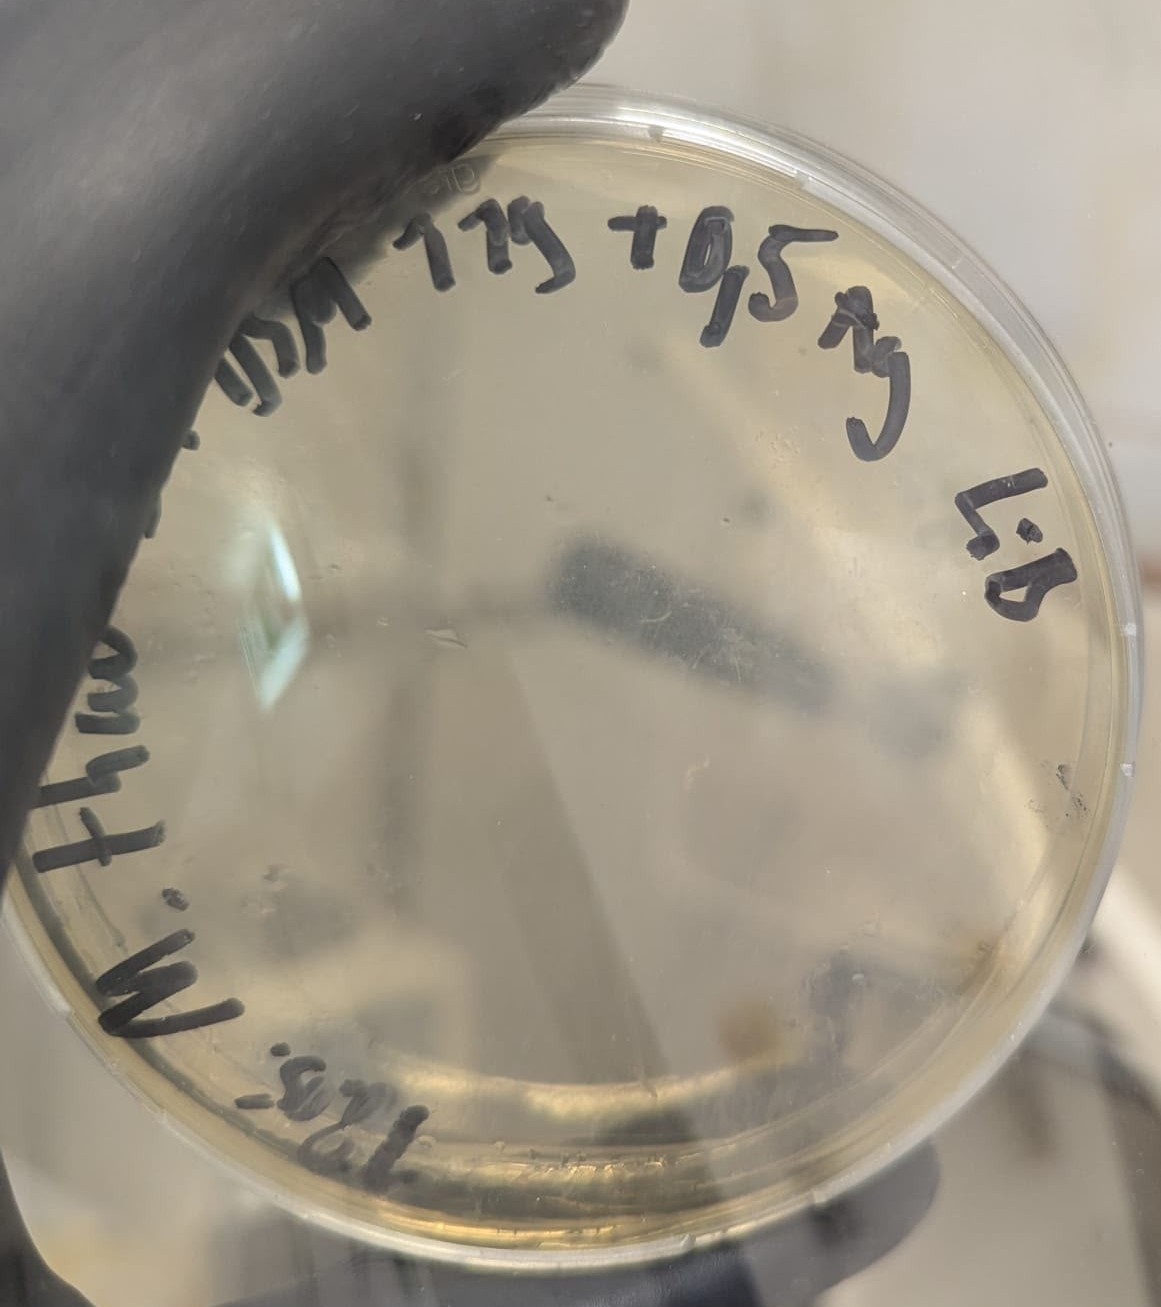
\includegraphics[width = 0.45\textwidth, height = 6cm]{figures/Results/BC/M_thau_pour_platin_119}
	\caption{Pour plating result of \acrfull{thau} DSM 119 (\textcolor{red}{1\% agar}). 100 µl of a full-grown culture have been plated. Cultivated in a jar with \ch{H2}/\ch{CO2} gas phase. No growth detected.}
	\label{fig:pour_plating}
\end{figure}


%%%%%%%%%%%%%%%%%%%%%%%%%%%%%%%%%%%%%%%%%%%%%%%%%%%%%%%%%%%%%%%%%%%%%%%%%%%%%%%%%%%%%%
%%%% Indicators for geodata analyses for all three countries

\begin{figure}[!h]
	\centering
	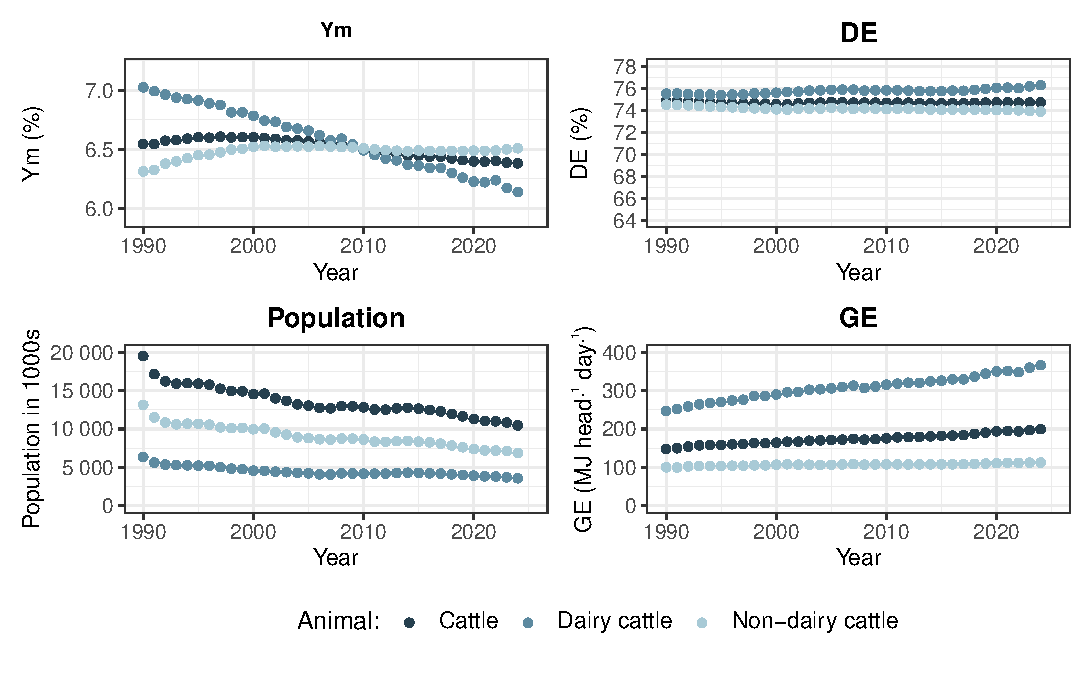
\includegraphics[width = \textwidth]{figures/Results/GEO/Indicitaor_plot_DEU.pdf}
	\caption{Time series of \acrfull{Ym}, \acrfull{DE}, population-size and \acrfull{GE} of cattle and its subcategories dairy and non-dairy for \acrlong{deu}.The data for dairy and non-dairy cattle is from the published \gls{crtglo}. The values for cattle is calculated as weighted mean of its subcategories, where the population-size is used as weight.}
	\label{fig:indic_deu}	
\end{figure}

\begin{figure}[!h]
	\centering
	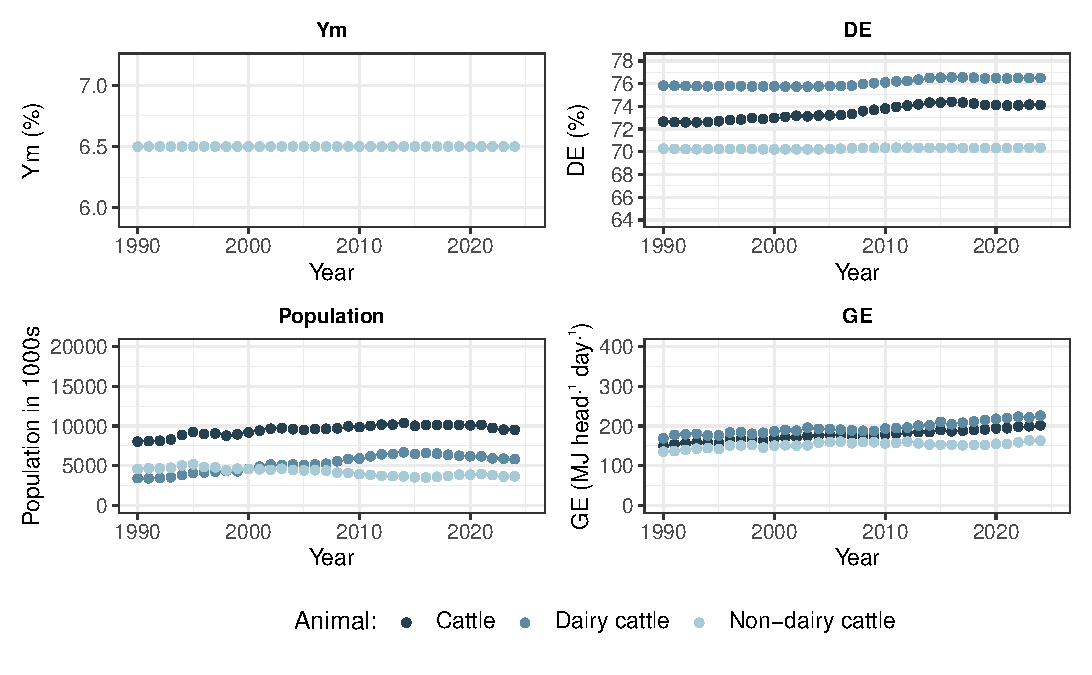
\includegraphics[width = \textwidth]{figures/Results/GEO/Indicitaor_plot_NZL.pdf}
	\caption{Time series of \acrfull{Ym}, \acrfull{DE}, population-size and \acrfull{GE} of cattle and its subcategories dairy and non-dairy for \acrlong{nzl}.The data for dairy and non-dairy cattle is from the published \gls{crtglo}. The values for cattle is calculated as weighted mean of its subcategories, where the population-size is used as weight.}
	\label{fig:indic_nzl}	
\end{figure}

\begin{figure}[!h]
	\centering
	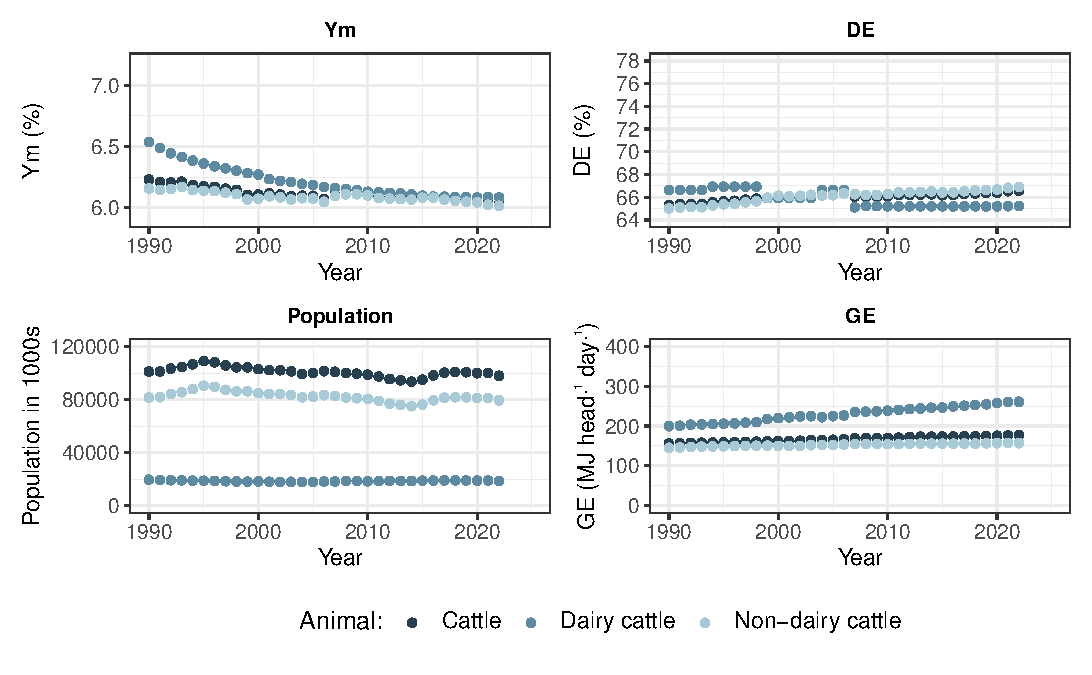
\includegraphics[width = \textwidth]{figures/Results/GEO/Indicitaor_plot_USA.pdf}
	\caption{Time series of \acrfull{Ym}, \acrfull{DE}, population-size and \acrfull{GE} of cattle and its subcategories dairy and non-dairy for \acrlong{usa}.The data for dairy and non-dairy cattle is from the published \gls{crtglo}. The values for cattle is calculated as weighted mean of its subcategories, where the population-size is used as weight.}
	\label{fig:indic_usa}	
\end{figure}
